\chapter*{Morphology-Density Appendix} \label{chap:morph_den_ap}

\section{Separation into SF \& Quiescent} \label{sec_c4:ap:cc_sel}

\begin{figure*}[htb]
    \centering
    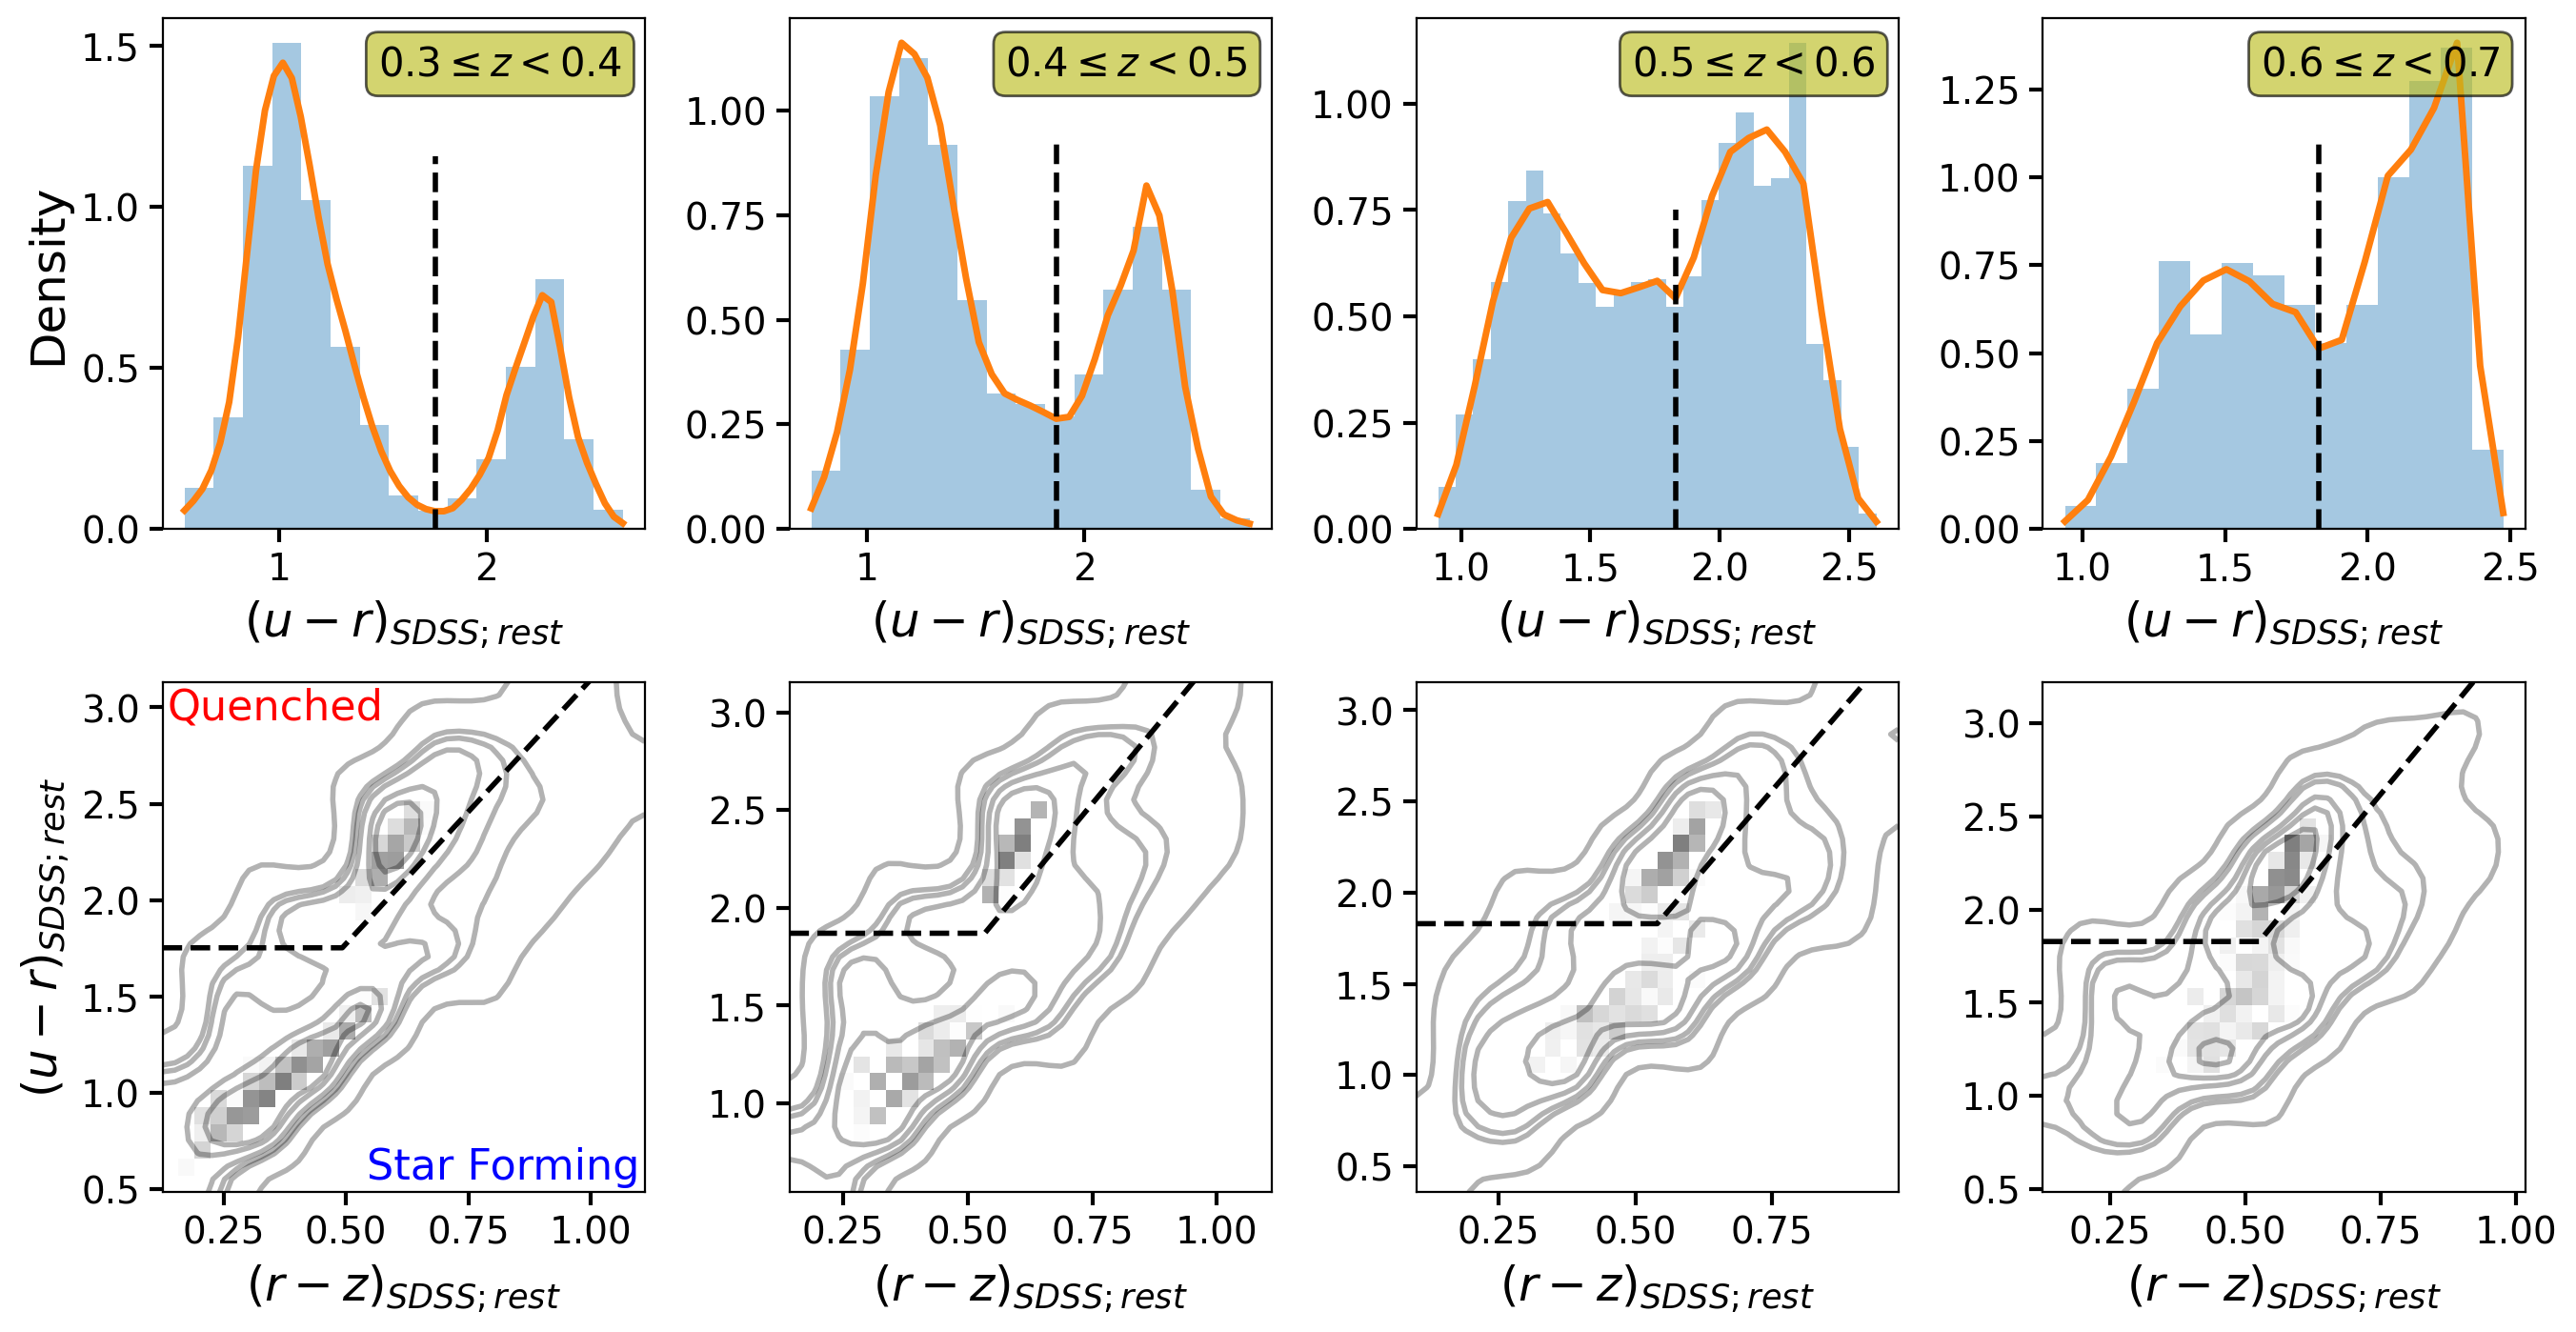
\includegraphics[width = \textwidth]{color_sep.png}
    \caption{Figure showing how we separate the galaxies in our sample into star-forming and quiescent sub-samples.}
    \label{fig_c4:color_sep}
\end{figure*}

To separate the galaxies in our sample into star-forming and quiescent sub-samples, we follow \citet{Kawin16} and \citet{hsc_mass_size}. We begin by defining a generic region on the \textit{urz} diagram for quiescent galaxies defined as 

\begin{equation}
    \begin{aligned}
        u-r & >A \times(r-z)+\mathrm{ZP} \\
        u-r & >(u-r)^{\prime} \\
        r-z & <1.15
\end{aligned}
\label{eq:color-color}
\end{equation}

where A, ZP, and $(u-r)^{\prime}$ are variables that we derive using galaxies in each redshift slice with stellar masses above the overall stellar mass completeness limit. 

\begin{table}[]
    \centering
    \caption{Best Fit Values For Eq. \ref{eq:color-color}  \label{tab_c4:color-color}}
    \begin{tabular}{cccc}
    \hline
    \hline
     Redshift Slice & $(u-r)^{\prime}$ & A & ZP \\
     \hline
     \hline
     $0.3 \leq z < 0.4$ & 1.75 & 2.75 & 0.40 \\
     $0.4 \leq z < 0.5$ & 1.87 & 3.07 & 0.23 \\
     $0.5 \leq z < 0.6$ & 1.83 & 3.48 & -0.05 \\
     $0.6 \leq z < 0.7$ & 1.83 & 3.52 & -0.02 \\
     \hline
     \hline
    \end{tabular}
\end{table}

First, we measure $(u-r)^{\prime}$ as the local minima between the two peaks observed in the u-r color distribution (see the upper panel of Figure \ref{fig_c4:color_sep}). Thereafter, we derive the value of A in Eq. \ref{eq:color-color} by fitting the slope of the red sequence in the \textit{urz} diagram. Once the slope of the line has been fixed, we now need to place it at an optimal location in the diagram. For this, we measure the \textit{urz} color distance of all galaxies from the line defined by the slope $A$ in Eq. \ref{eq:color-color}. Finally, we set zero-point $ZP$ to be the local minima between the two peaks in the measured \textit{urz} color distance distribution. 

The bottom panels of Figure \ref{fig_c4:color_sep} show the final separation boundaries obtained for each redshift slice. The final fitted values for all the parameters in Eq. \ref{eq:color-color} are also shown in Table \ref{tab_c4:color-color}. We refer the interested reader to \citet{Kawin16} for a more extended description of the above procedure. 

%\section{Effect of Color Gradients on Our Results} \label{sec_c4:ap:size_corr}

%Discuss the results of using the corrected sizes and using them in our analysis. 


\section{Correlation Coefficients \label{sec_c4:ap:corr_coeff}}

The full version of Table \ref{tab_c4:corr_subpop_ab} is shown here as Table \ref{tab_c4:corr_subpop}. 

\newpage
\begin{landscape}
\begin{table*}[htbp]
\centering
\caption{Statistical Significance of Radius v/s Density Correlations for Galaxy Sub-Populations \label{tab_c4:corr_subpop}}
\begin{tabular}{c|c|c|cccc}
\hline
\hline
Sub-Population & Mass Range & & $0.3 \leq z < 0.4$ & $0.4 \leq z < 0.5$ & $0.5 \leq z < 0.6$ & $0.6 \leq z < 0.7$ \\ 
          & ($\log M/M_{\odot}$) & & & & \\
\hline
\hline
\multirow{8}{*}{Disk-Dominated} & \multirow[c]{4}{*}{$\geq10.25$} & $\rho$   & $4.8\times10^{-2} \pm 9.6\times10^{-4}$ & $7.7\times10^{-2} \pm 8.6\times10^{-4}$ & $1.9\times10^{-2} \pm 4\times10^{-4}$ & $1.7\times10^{-2} \pm 4\times10^{-4}$ \\
                                    &                                     & $p$      & $1.2\times10^{-13} \pm 4\times10^{-13}$ & $4\times10^{-101} \pm 9.5\times10^{-95}$ & $1.8\times10^{-9} \pm 2.2\times10^{-9}$ &  $3.3\times10^{-8} \pm 3.2\times10^{-8}$   \\
                                    & & $\alpha$ & $49\sigma_{\rho}$ & $89\sigma_{\rho}$ & $47\sigma_{\rho}$ & $44\sigma_{\rho}$  \\
                                    & & $>5\sigma$ & \checkmark & \checkmark &  Borderline \checkmark &  Borderline \checkmark \\
                 \cline{2-7}
                 & \multirow[c]{4}{*}{$<10.25$} & $\rho$   & $6.4\times10^{-2} \pm 5.0\times10^{-4}$ & $1.1\times10^{-1} \pm 5.7\times10^{-4}$ & $1.6\times10^{-2} \pm 4.8\times10^{-4}$ & $7.7\times10^{-3} \pm 5.1\times10^{-4}$ \\
                                    &             & $p$      & $2.5\times10^{-92} \pm 6.4\times10^{-89}$ & $3.6\times10^{-252} \pm (<10^{-300})$ & $8.3\times10^{-7} \pm 9.9\times10^{-7}$ &  $1.5\times10^{-2} \pm 7.5\times10^{-3}$   \\
                                    & & $\alpha$ & $127\sigma_{\rho}$ & $188\sigma_{\rho}$ & $32\sigma_{\rho}$ & $14\sigma_{\rho}$  \\
                                    & & $>5\sigma$ & \checkmark & \checkmark &  &  \\
    \hline
    \hline
    \multirow{8}{*}{Star-Forming} & \multirow[c]{4}{*}{$\geq10.25$}       & $\rho$   & $7.3\times10^{-2} \pm 1.5\times10^{-3}$ & $1\times10^{-1} \pm 9.5\times10^{-4}$ & $3.2\times10^{-2} \pm 8.2\times10^{-4}$ & $1.7\times10^{-2} \pm 4.3\times10^{-4}$ \\
                                    &                                     & $p$      & $2.5\times10^{-18} \pm 2.1\times10^{-17}$ & $4.4\times10^{-160} \pm 3\times10^{-152}$ & $1.7\times10^{-20} \pm 8.3\times10^{-19}$ &  $3.7\times10^{-8} \pm 4.4\times10^{-8}$   \\
                                    &                                     & $\alpha$ & $48\sigma_{\rho}$ & $109\sigma_{\rho}$ & $39\sigma_{\rho}$ & $40\sigma_{\rho}$  \\
                                    & & $>5\sigma$ & \checkmark & \checkmark & \checkmark &  Borderline \checkmark \\
                 \cline{2-7}
                 & \multirow[c]{4}{*}{$<10.25$} & $\rho$   & $8.7\times10^{-2} \pm 5.7\times10^{-4}$ & $1\times10^{-1} \pm 6.8\times10^{-4}$ & $2.8\times10^{-2} \pm 5\times10^{-4}$ & $1.4\times10^{-2} \pm 5.4\times10^{-4}$ \\
                                    &             & $p$      & $4.6\times10^{-169} \pm (<10^{-300})$ & $1.4\times10^{-242} \pm (<10^{-300})$ & $3.7\times10^{-19} \pm 2.2\times10^{-18}$ &  $1.8\times10^{-5} \pm 2\times10^{-5}$   \\
                                    & & $\alpha$ & $152\sigma_{\rho}$ & $154\sigma_{\rho}$ & $57\sigma_{\rho}$ & $24\sigma_{\rho}$  \\
                                    & & $>5\sigma$ & \checkmark & \checkmark & \checkmark &  \\
    \hline
    \hline
    \multirow{8}{*}{Bulge-Dominated} & \multirow[c]{4}{*}{$\geq10.25$} & $\rho$   & $1.3\times10^{-1} \pm 9.6\times10^{-4}$ & $1.1\times10^{-1} \pm 9\times10^{-4}$ & $5.2\times10^{-2} \pm 1.1\times10^{-3}$ & $2.9\times10^{-2} \pm 5.3\times10^{-4}$ \\
                                    &                                     & $p$      & $1.8\times10^{-155} \pm 1.9\times10^{-149}$ & $1.3\times10^{-167} \pm 1.3\times10^{-157}$ & $1.3\times10^{-42} \pm 1.3\times10^{-38}$ &  $1.2\times10^{-20} \pm 1.0\times10^{-19}$   \\
                                    & & $\alpha$ & $136\sigma_{\rho}$ & $118\sigma_{\rho}$ & $47\sigma_{\rho}$ & $55\sigma_{\rho}$  \\
                                    & & $>5\sigma$ & \checkmark & \checkmark &  \checkmark &  \checkmark \\
                 \cline{2-7}
                 & \multirow[c]{4}{*}{$<10.25$} & $\rho$   & $1.1\times10^{-1} \pm 1.3\times10^{-3}$ & $6.1\times10^{-2} \pm 1.5\times10^{-3}$ & $5.3\times10^{-2} \pm 1.7\times10^{-3}$ & $3.6\times10^{-4} \pm 1.4\times10^{-3}$ \\
                                    &             & $p$      & $1.3\times10^{-102} \pm 1.4\times10^{-94}$ & $8.2\times10^{-38} \pm 6\times10^{-34}$ & $1.4\times10^{-25} \pm 8.2\times10^{-22}$ &  $8.2\times10^{-1} \pm 1.5\times10^{-1}$   \\
                                    & & $\alpha$ & $79\sigma_{\rho}$ & $40\sigma_{\rho}$ & $30\sigma_{\rho}$ & 0  \\
                                    & & $>5\sigma$ & \checkmark & \checkmark & \checkmark &  \\
    \hline
    \hline
    \multirow{8}{*}{Quiescent} & \multirow[c]{4}{*}{$\geq10.25$} & $\rho$   & $1.1\times10^{-1} \pm 6.5\times10^{-4}$ & $1\times10^{-1} \pm 5.3\times10^{-4}$ & $3.8\times10^{-2} \pm 4.1\times10^{-4}$ & $3.3\times10^{-2} \pm 4.2\times10^{-4}$ \\
                                    &                                     & $p$      & $1.6\times10^{-197} \pm (<10^{-300})$ & $5.1\times10^{-229} \pm (<10^{-300})$ & $1.6\times10^{-32} \pm 1.4\times10^{-31}$ &  $5.9\times10^{-25} \pm 3.3\times10^{-24}$   \\
                                    & & $\alpha$ & $177\sigma_{\rho}$ & $192\sigma_{\rho}$ & $92\sigma_{\rho}$ & $77\sigma_{\rho}$  \\
                                    & & $>5\sigma$ & \checkmark & \checkmark &  \checkmark &  \checkmark \\
                 \cline{2-7}
                 & \multirow[c]{4}{*}{$<10.25$} & $\rho$   & $1.5\times10^{-1} \pm 1\times10^{-3}$ & $1.3\times10^{-1} \pm 9.8\times10^{-4}$ & $4.1\times10^{-2} \pm 1.2\times10^{-3}$ & $2.3\times10^{-2} \pm 1.2\times10^{-3}$ \\
                                    &             & $p$      & $1.9\times10^{-259} \pm (<10^{-300})$ & $2.2\times10^{-241} \pm (<10^{-300})$ & $9.7\times10^{-29} \pm 1\times10^{-24}$ &  $1.1\times10^{-11} \pm 8.3\times10^{-10}$   \\
                                    & & $\alpha$ & $153\sigma_{\rho}$ & $134\sigma_{\rho}$ & $33\sigma_{\rho}$ & 18$\sigma_{\rho}$  \\
                                    & & $>5\sigma$ & \checkmark & \checkmark & \checkmark & Borderline \checkmark \\
    \hline
    \hline
\end{tabular}    
\end{table*}
\end{landscape}
\newpage